\section{MIF with Magnetic Mirrors: Feasibility Analysis}

The feasibility of a fusion concept should be one of the first considerations in its development. The purpose of this investigation, is to determine if the MIF with magnetic mirror approach presented in this report is scientifically feasible i.e. that the required parameters to reach $Q$ = 1 (net power divided by the power supplied to the plasma), are realistically achievable. Other relevant metrics are the required ignition conditions and scalability.

A key parameter to assess the performance of a fusion concept is the Lawson criterion. This criterion, developed by John D. Lawson in the 1950s, essentially determines whether a fusion system can produce net energy. It posits that the product of plasma density ($n$), temperature ($T_i$), and confinement time ($\tau$) must exceed a certain threshold for a fusion reactor to generate more energy than it consumes ($Q > 1$) \cite{mills1971lawson}. The specific range of each of these parameters varies between concepts, but a triple product of $>10^{22}$ is generally approaching the region of net gain and commercial relevance. The achieved Lawson parameters vs $T_i$ is plotted for various MCF, MIF and IFE experiments in figure \ref{fig:wurzel}.

\begin{figure}[h!]
    \centering
    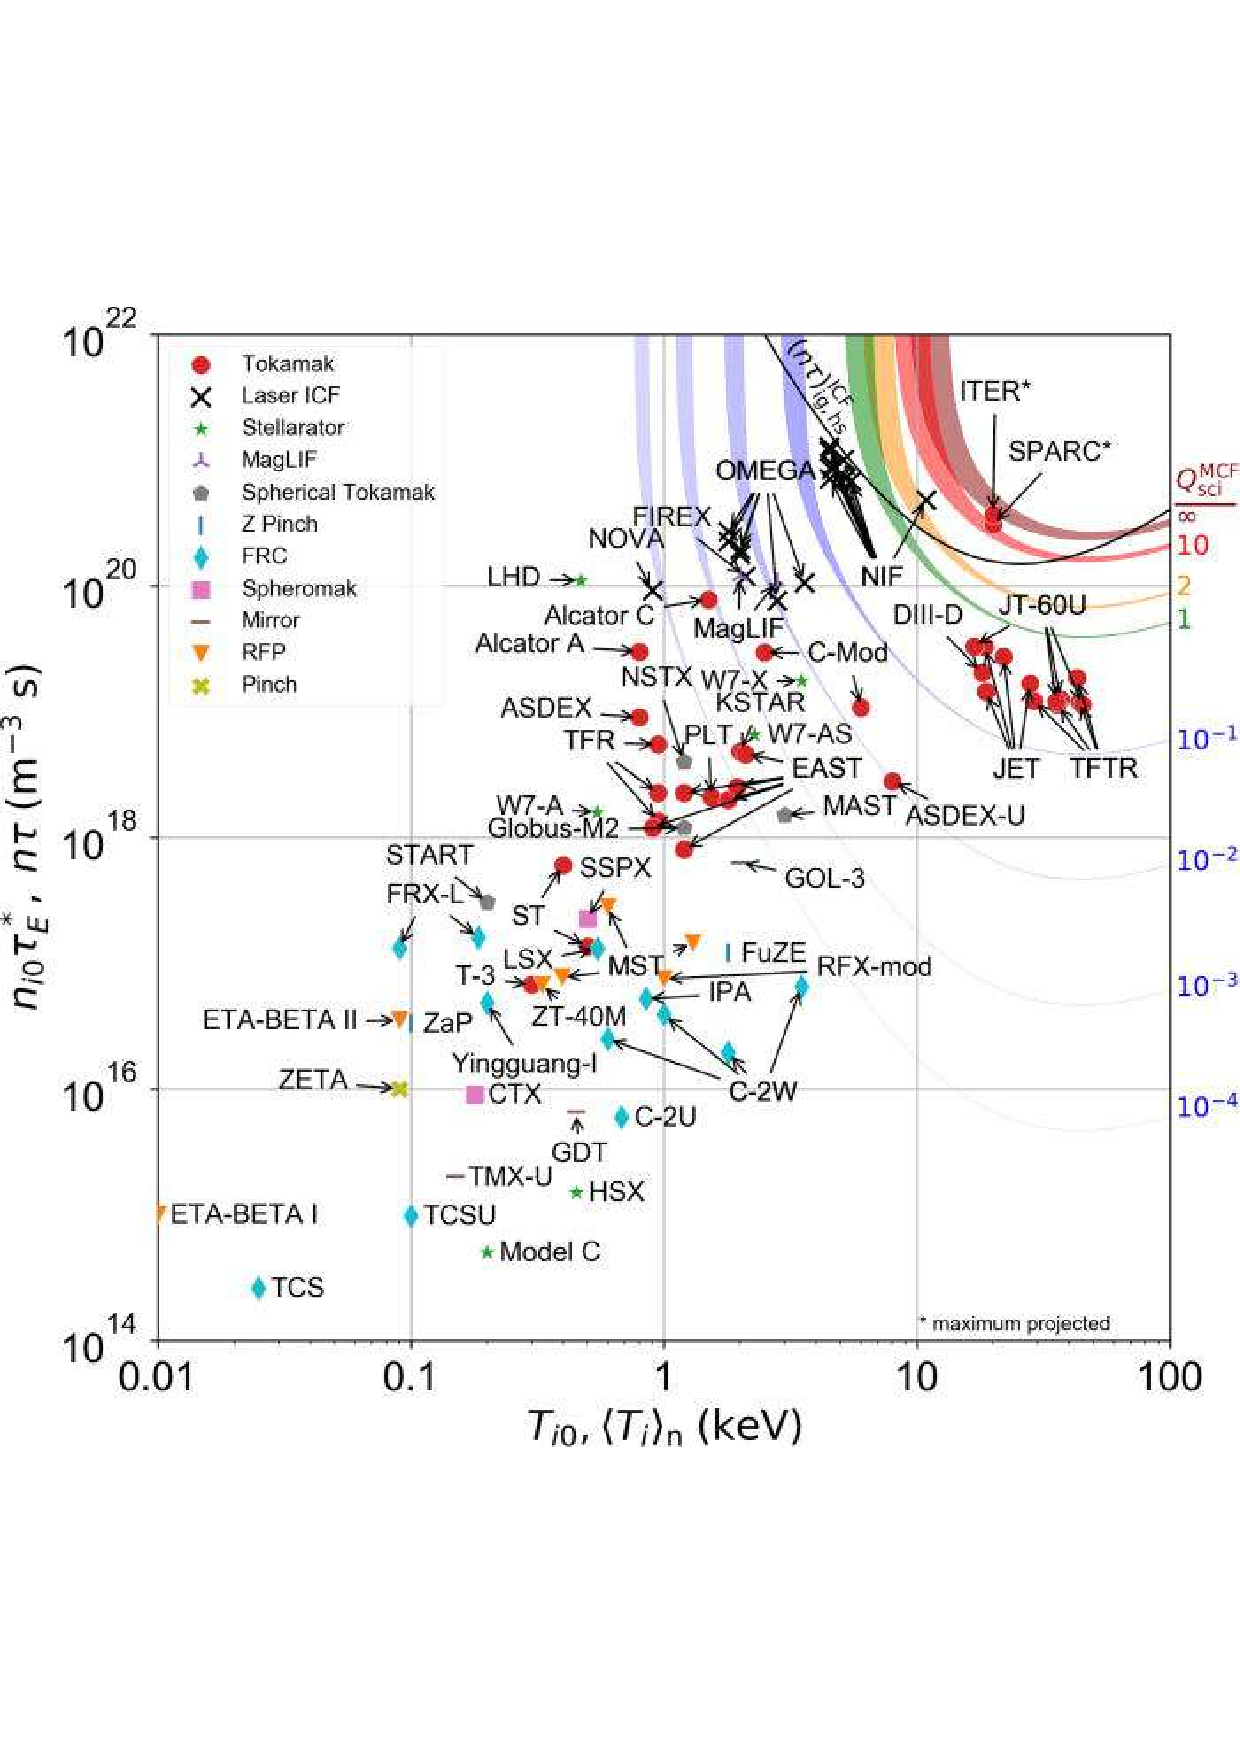
\includegraphics[width=0.8\linewidth]{SubreportFigures/wurzel_fusion_nttau.pdf}
    \caption{Experimentally inferred Lawson parameters for MCF, IFE and MIF. From \cite{wurzel2022progress}.}
    \label{fig:enter-label}
\end{figure}


Although the triple product must be approximately $>10^{21}$, the individual values of $n$, $T_i$ and $\tau$ can vary considerably between concepts and confinement types:

\begin{itemize}
    \item Magnetic Confinement Fusion (MCF): This method typically uses lower plasma densities. In devices like tokamaks or stellarators, the plasma density is usually in the range of 10$^{17}$ to 10$^21$ particles per cubic meter \cite{brezinsek2019mcf}.
\item Inertial Confinement Fusion (IFE): IFE achieves extremely high densities, often several orders of magnitude higher than MCF, in the range of 10$^{27}$ to 10$^32$ to particles per cubic meter during the brief confinement period \cite{brezinsek2019mcf}.
\item Magnetized Inertial Fusion (MIF): MIF, which includes concepts like magnetic mirror approaches, occupies an intermediate density range between MCF and IFE. It aims to leverage the benefits of both magnetic and inertial confinement, potentially allowing for more practical and feasible fusion conditions.
\end{itemize}

For the concept considered here, $n \approx 10^{21}$ is reasonable. For $T_i$, and $\tau$ recent temperature measurements at the Maryland Centrifugal experiment observed thermal electron temperatures in excess of 100 eV, and a confinement time, $\tau$ of $5.9 \pm 1.6 \times 10^{-4}$ seconds \cite{reid2014100}.  

In the magnetic mirror fusion (MIF) concept presented in this report, a plasma density (\(n\)) of approximately \(10^{21}\) particles per cubic meter is achievable. Experiments like those at the Maryland Centrifugal Experiment have recorded thermal electron temperatures over 100 eV, with a confinement time (\(\tau\)) of \(5.9 \pm 1.6 \times 10^{-4}\) seconds \cite{reid2014100}. \(\tau\) is an important parameter in fusion theory, indicating how long plasma is confined and hot enough to sustain nuclear fusion reactions. In magnetic mirror fusion, the effectiveness of magnetic fields in confining plasma and reducing energy loss significantly affects \(\tau\). Longer confinement time is linked to better conditions for fusion ignition. Modeling of \(\tau\), along with other parameters during plasma compression, reveals that \(\tau\) in this case aligns with Ohmic confinement scaling.

Ohmic heating significantly influences plasma confinement and heating in magnetic mirror fusion. Ohmic confinement scaling, arising from plasma interactions with electric currents and magnetic fields, aids in evaluating plasma confinement efficiency \cite{bessenrodt1991multiple}. This scaling law clarifies how confinement time varies with changes in plasma density, temperature, and magnetic field strength. Understanding this relationship is important for refining magnetic mirror fusion designs, particularly in the context of confinement time (\(\tau\)) as discussed in this report.

As a first approximation, an analytical approach is sufficient. For this MIF design, the convergence ratio, $C_r$ of the plasma is critical \cite{ellis2001experiment}. This is the ratio of the initial to final plasma radius due to compression, and from this, along with $n$, $T_i$ and $\tau$, a yield can be calculated for fission neutrons and alpha particles. From \cite{reid2014100}, the power supplied to the plasma, $P_{in}$ was $5.8 \pm 0.42$ MW, so using $Q = P_e/P_{in}$, where $P_e$ is the fusion energy, an approximation of the yield for various parameter values can be obtained. 


 Using the values from \cite{reid2014100} as a reference point, each $n$, $T_i$,$\tau$ and $C_r$ can be varied to find an achievable parameter space in reality. The results of a 3D parameter sweep, performed in this way can be seen in \ref{fig:model_3d_1}. It can be seen from this model that by achieving approximately; $n > 1.5 \times 10^{20}$, $C_r > 2.9$, and $T_0 > 110$ eV, $Q > 1$ can be achieved ($Q > 1$ is still achievable with different parameter values, this is just a reasonable example). 

\begin{figure}[h!] 
\centering
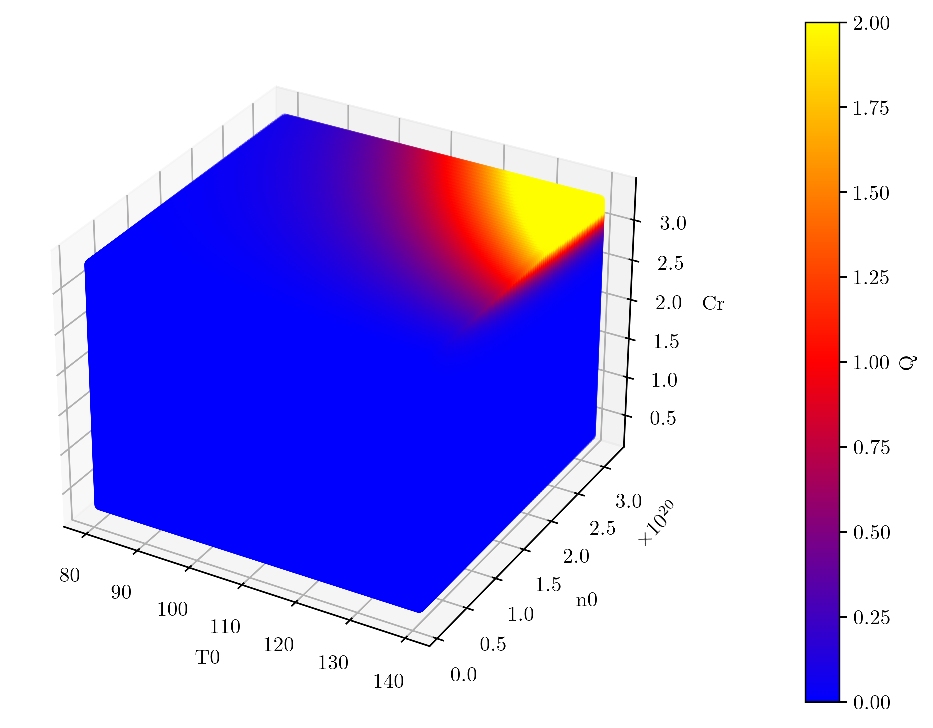
\includegraphics[scale=0.51]{SubreportFigures/Q_n0_T0_Cr_1_3d.pdf}
\caption{MIF parameter space from physics model, where $Q = 1$ can be achieved.}
\label{fig:model_3d_1}
\end{figure}

In the scenario that a larger initial plasma radius can be established, for example with a larger machine, the parameter space in $C_r$ can be extended, opening up larger $Q$ values. The results of such a sweep can be seen in figure \ref{fig:model_3d_10}. A $Q > 10$ can be achieved with, for example an initial plasma radius of 0.6 m, and a final radius of 0.15 m, without significant increases being required for the other relevant parameters.

\begin{figure}[h!] 
\centering
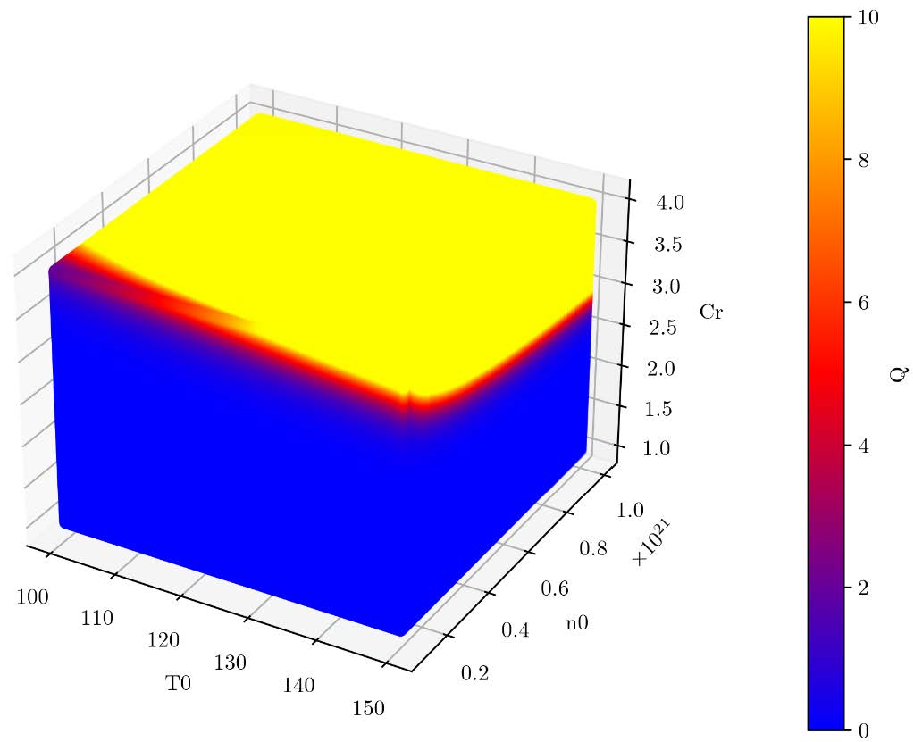
\includegraphics[scale=0.5]{SubreportFigures/Q_n0_T0_Cr_10_3d.pdf}
\caption{MIF parameter space from physics model, where $Q = 10$ can be achieved..}
\label{fig:model_3d_10}
\end{figure}

To summarise, the values of key parameters $n$, $T_i$,$\tau$ and $C_r$ were determined and varied within realistically achievable ranges to identify the required parameter space to obtain net gain, $Q > 1$. It is found that, based on an analytical approach using Ohmic scaling, the conditions required to obtain net gain is within reasonable iteration of existing experiments, and that the design parameters presented for the concept in this report are considerably beyond what would be required for $Q > 10$.